\section{Apendice}

\subsection{Requerimientos del software}
Para poder utilizar el parser es necesario contar con el interprete de python
(cualquier version de 2.7 en adelante), que puede instalarse desde cualquier
terminal linux mediante el comando:

\begin{verbatim}
$ apt-get install python2.7
\end{verbatim}

o descargandolo de su pagina oficial : \url{https://www.python.org/}. \\
Tambien es necesario contar con la herramienta PLY(cualquier version de 3.6 en
adelante) de python, la cual puede ser
instalada una vez que se cuente con el interprete de python mediante el siguiente comando en la terminal.
\begin{verbatim}
$ pip install ply
\end{verbatim}
o descargandolo de su pagina oficial \url{http://www.dabeaz.com/ply/}

\subsection{Modo de Uso}
Para ejecutar el parser debe ejecutarse en una terminal de linux el siguiente
comando desde la carpeta donde se encuentra el codigo:
\begin{verbatim}
$ ./SLSParser -c INPUT -o OUTPUT
\end{verbatim}


En donde INPUT sera el path del archivo a parsear y OUTPUT el path en donde
sera escrito el resultado del parser luego de aplicar las reglas.

En caso de no
especificar un archivo de entrada el parser funcionara de forma interactiva,
permitiendo al usuario escribir en la terminal el codigo que desea parsear. Una
vez que el usuario termina de escribir manualmente lo que desea parsear debera
presionar CTRL+d, con lo cual se ejecutara el parser y mostrara por pantalla
los resultados obtenidos.

\subsection{Código}
A continuación presentamos el codigo utilizado para generar las reglas del
parser y del lexer, junto con las clases utilizadas para
la traduccion dirigida por sintaxis. Tambien presentaremos los tokens y los
tokens reservados.
\subsubsection{Reglas del parser}
\lstinputlisting{../src/parser_rules.py}

\subsubsection{Reglas del lexer}
\lstinputlisting{../src/lexer_rules.py}

\subsubsection{Clases utilizadas}
\lstinputlisting{../src/expression.py}

\subsubsection{Tokens y palabras reservadas}
\lstinputlisting{../src/tokens.py}




\subsection{Enunciado}
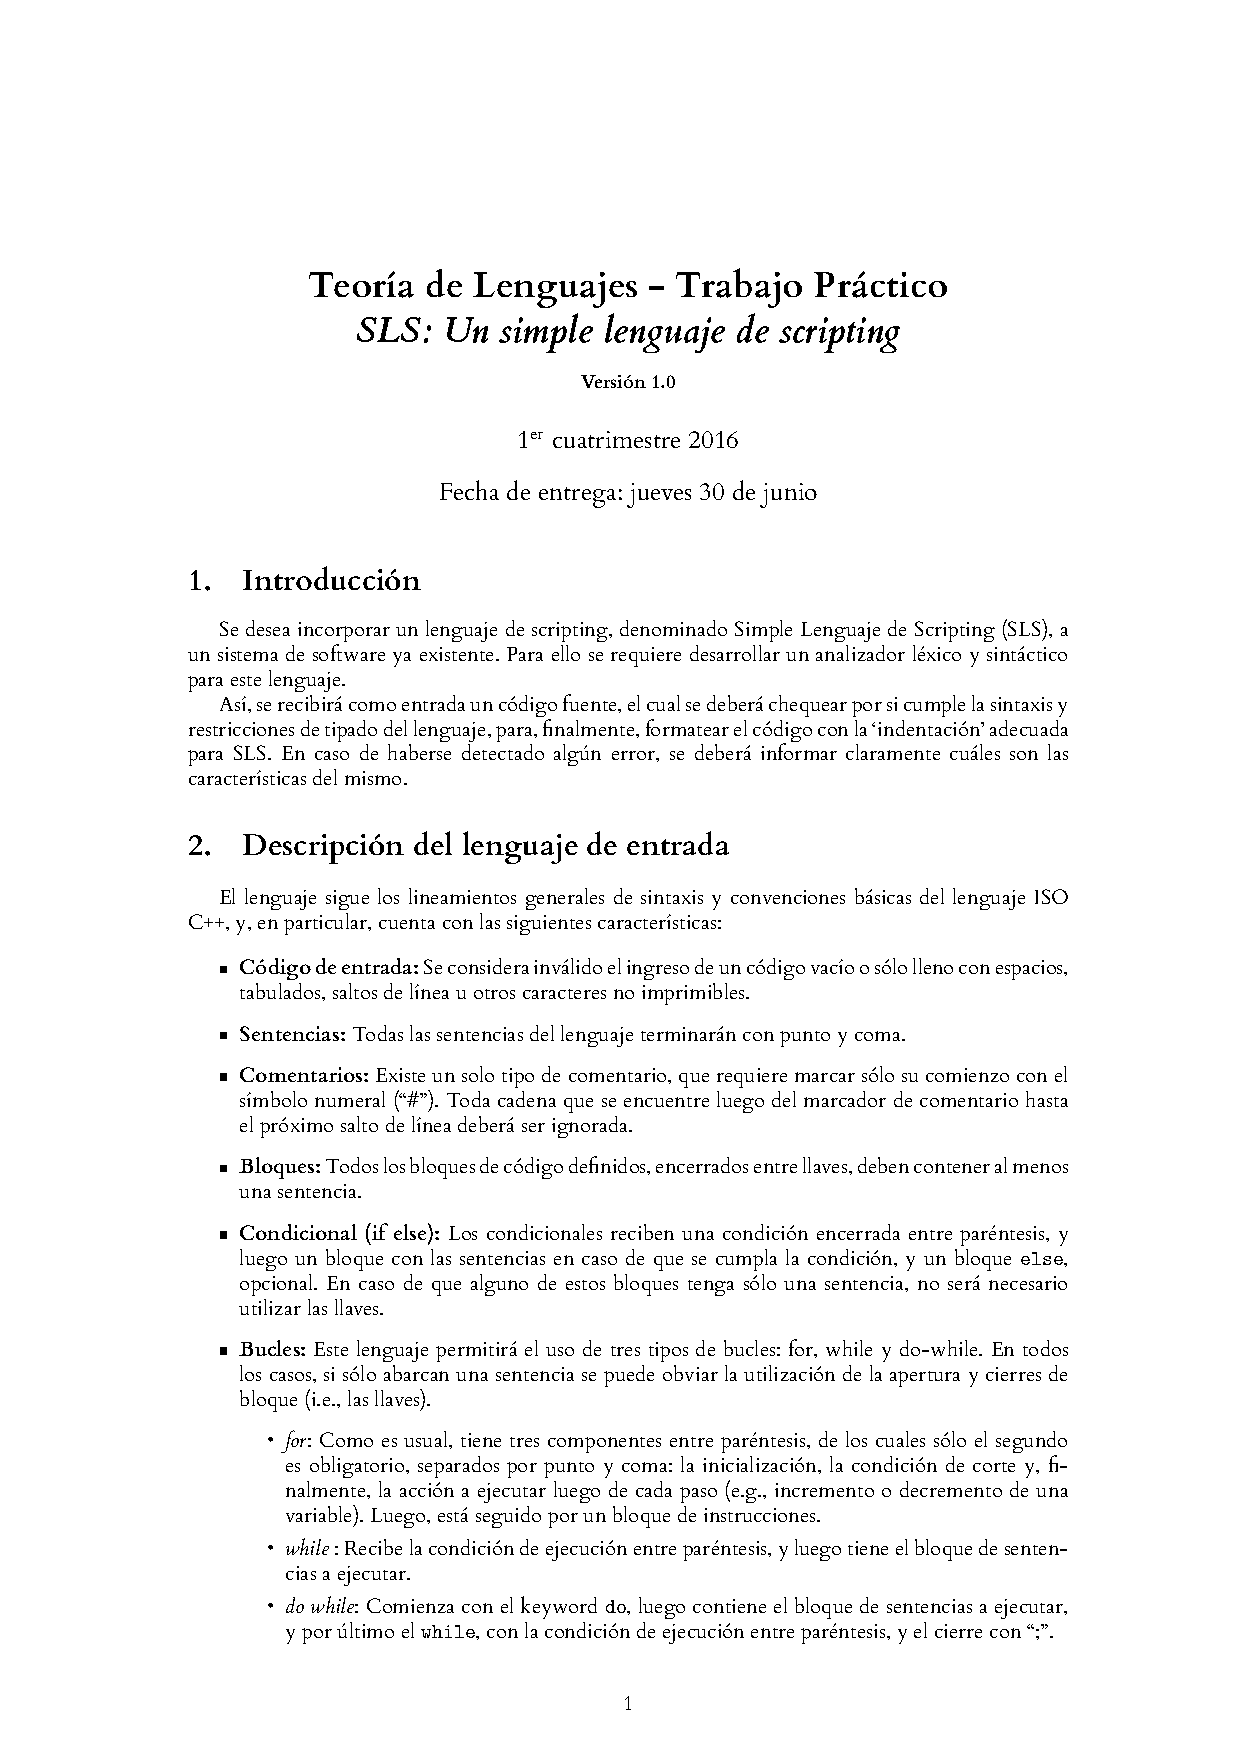
\includepdf[pages=-]{../enunciado/enunciado.pdf}
